\subsection{常用术语}
为方便理解,本设计中部分常见术语规定如下,具体设计中如有特殊术语或图例已在图中绘制图例,此处不再赘述。

\begin{description}
  \item [凝视触发] 通过凝视某个控件使其触发,常用于按钮、方向控件等
  \item [指向图标] 全景漫游用于进行场景切换的图标标识
\end{description}

\subsubsection{方位定义}
全景漫游中漫游的主体是一台虚拟的摄像机,整个呈现的场景都是它所拍摄的画面。根据机械原理,一个物体具有 6 个方向的自由度。以右手坐标系为基准,三个正交轴轴分别为 xyz,则其中一个物体的自由度分别是 xyz 三个轴方向上的位移及绕这三个轴的转角,如图\ref{fig:d-13}。当进行场景漫游时,其实就是通过调整这 6 个自由度中的一个或多个,继而改变场景画面\endnote{Ritchey K J. Panoramic image based virtual reality/telepresence audio-visual system and method: US, US 20080024594 A1[P]. 2008.}。

其中,三个轴的转角是通过重力感应器来捕捉动作并进行调整,而三个轴上的位移则需要额外的输入形式,但考虑到物理真实的需要,一般不做 y 轴方向(即重力方向)的位移,故只需进行 xz 两轴的位移,下文提到的位置控件即是实现了在场景内水平方向的漫游功能。

\begin{figure}[htp]
\centering
\fbox{
  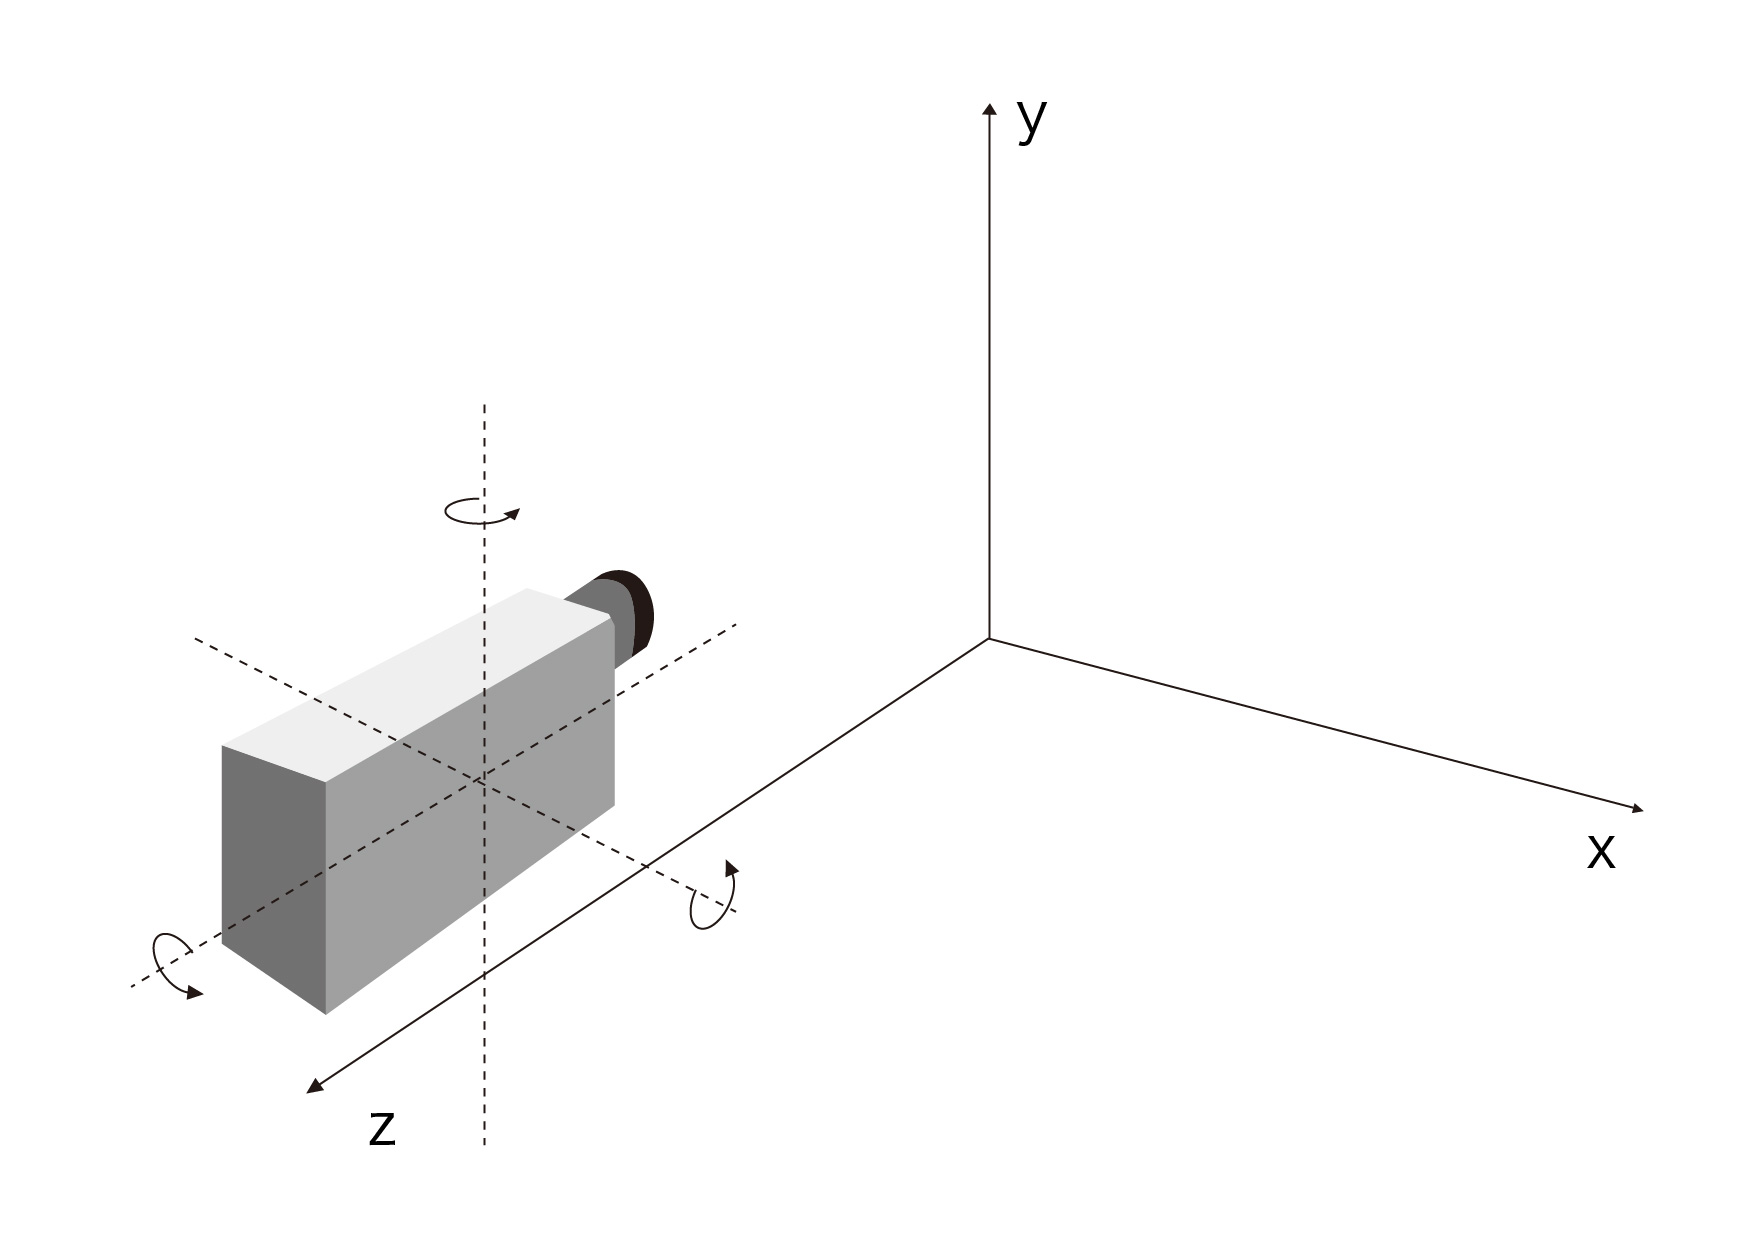
\includegraphics[width=.5\textwidth]{design/d-13}
}
\caption{全景漫游的 6 个自由度}
\label{fig:d-13}
\end{figure}

\subsection{导航界面设计}
导航功能试图在单个界面里包容更多的上下文信息以便用户准确定位自身所在,同时通过多界面并存的形式方便用户可以随时查看早前访问过的页面。根据前文人的视域的特性,导航界面整体功能菜单向下布置,主要元素垂直方向布置,方便用户浏览。因全景漫游具有一定的空间感,将部分界面设计成多面环状排布更有利于用户查看相关信息。

导航漫游记录以 3D 界面形式呈现。用户可由当前界面观察到早先访问过的界面的一部分,有助于用户建立上下文感知。如图\ref{fig:d-03}。

\begin{figure}[htp]
\centering
\fbox{
  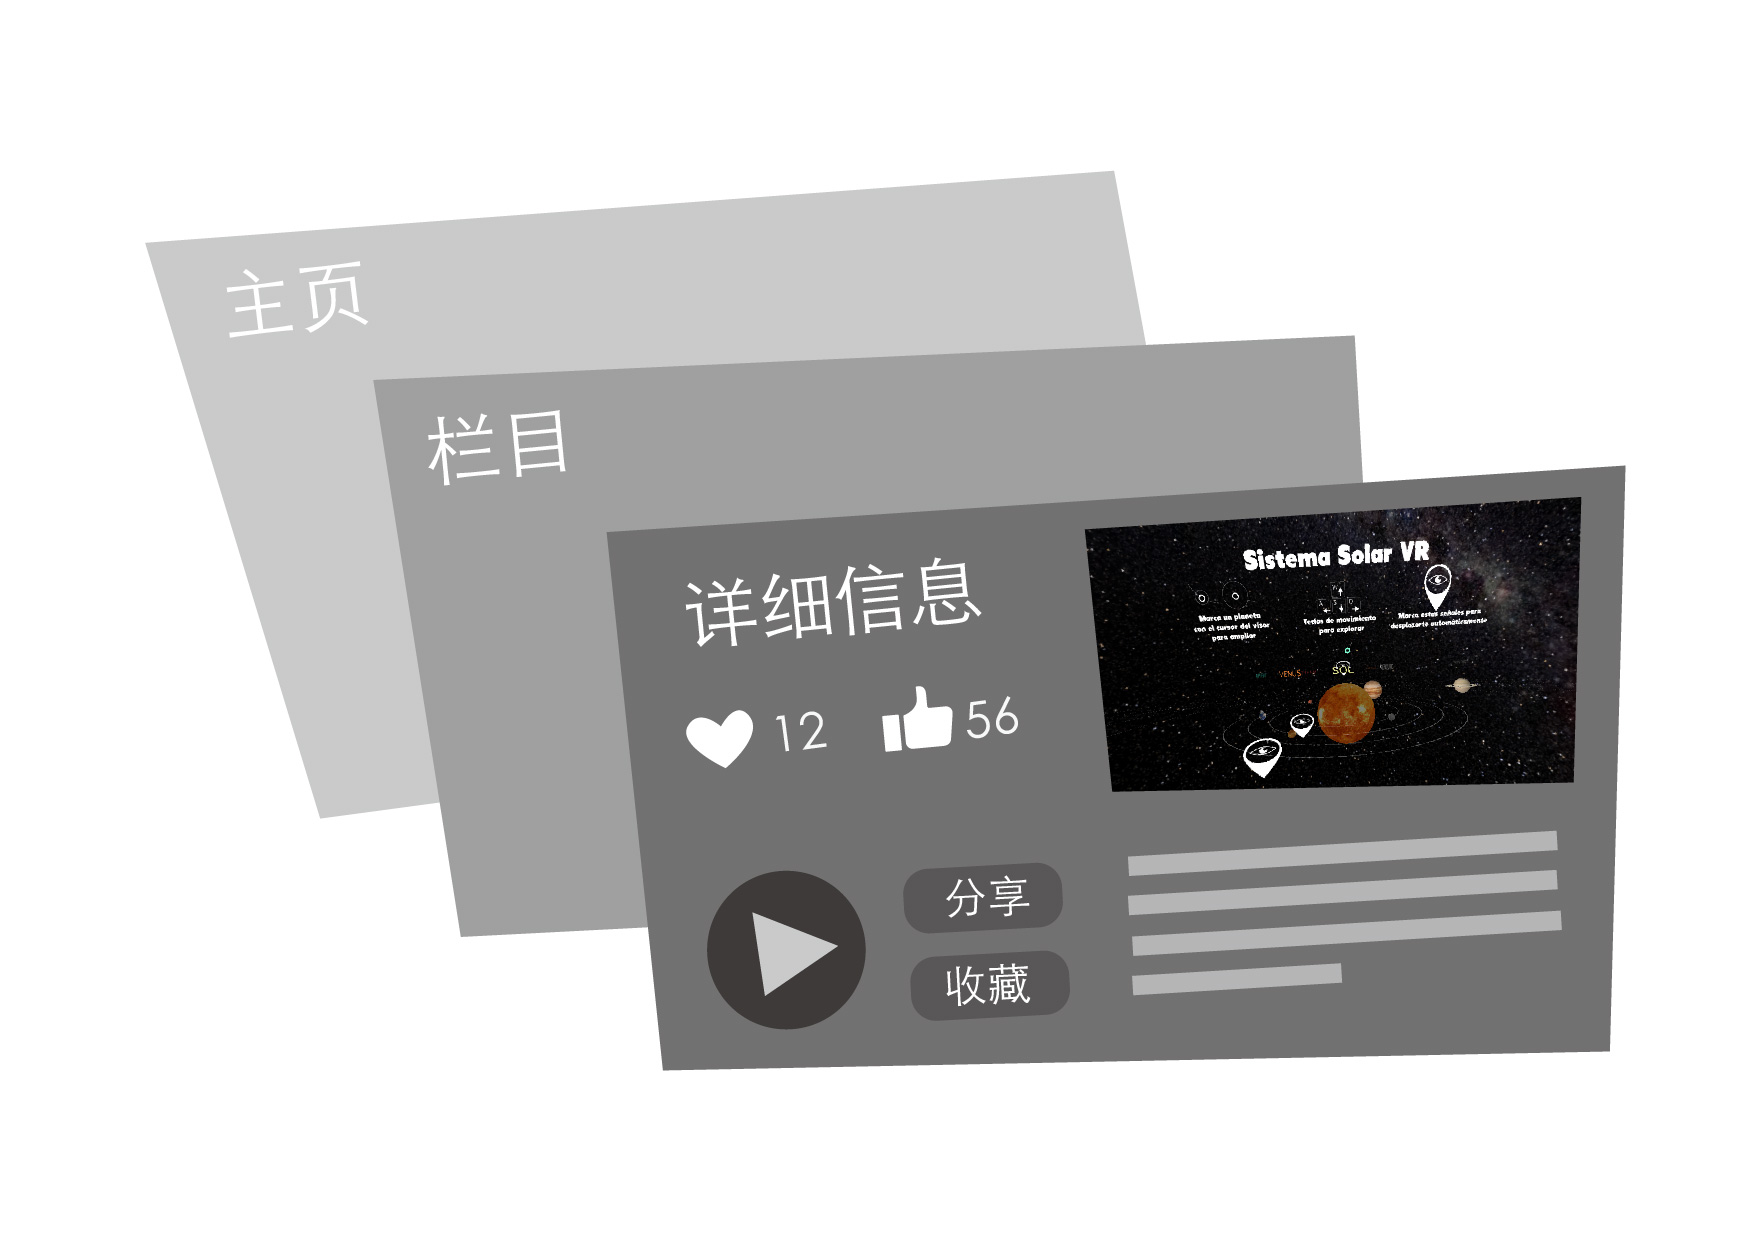
\includegraphics[width=.5\textwidth]{design/d-03}
}
\caption{3D界面}
\label{fig:d-03}
\end{figure}

\subsubsection{主界面}
主界面采用格式塔法则将各功能元素按区块设置。根据视觉特性,人的视觉注意是从左上至右上,再从左下至右下。中心界面左上为推荐模块,是用户进入界面后第一眼看到的场景,最容易吸引用户注意力。右上方为类别菜单,帮助用户建立漫游系统的分类体系。整个下方为二级推荐栏目,这里是系统根据用户特征及热门栏目综合计算得出的推荐项目。

左侧界面为部分置顶的类别界面,下方为标签栏,提供给用户切换分类的功能,用户可以通过浏览上部菜单了解到该类别部分场景的信息。右侧界面为历史记录或收藏夹界面。

主界面设计如图\ref{fig:d-01}。

\begin{figure}[htp]
\centering
\fbox{
  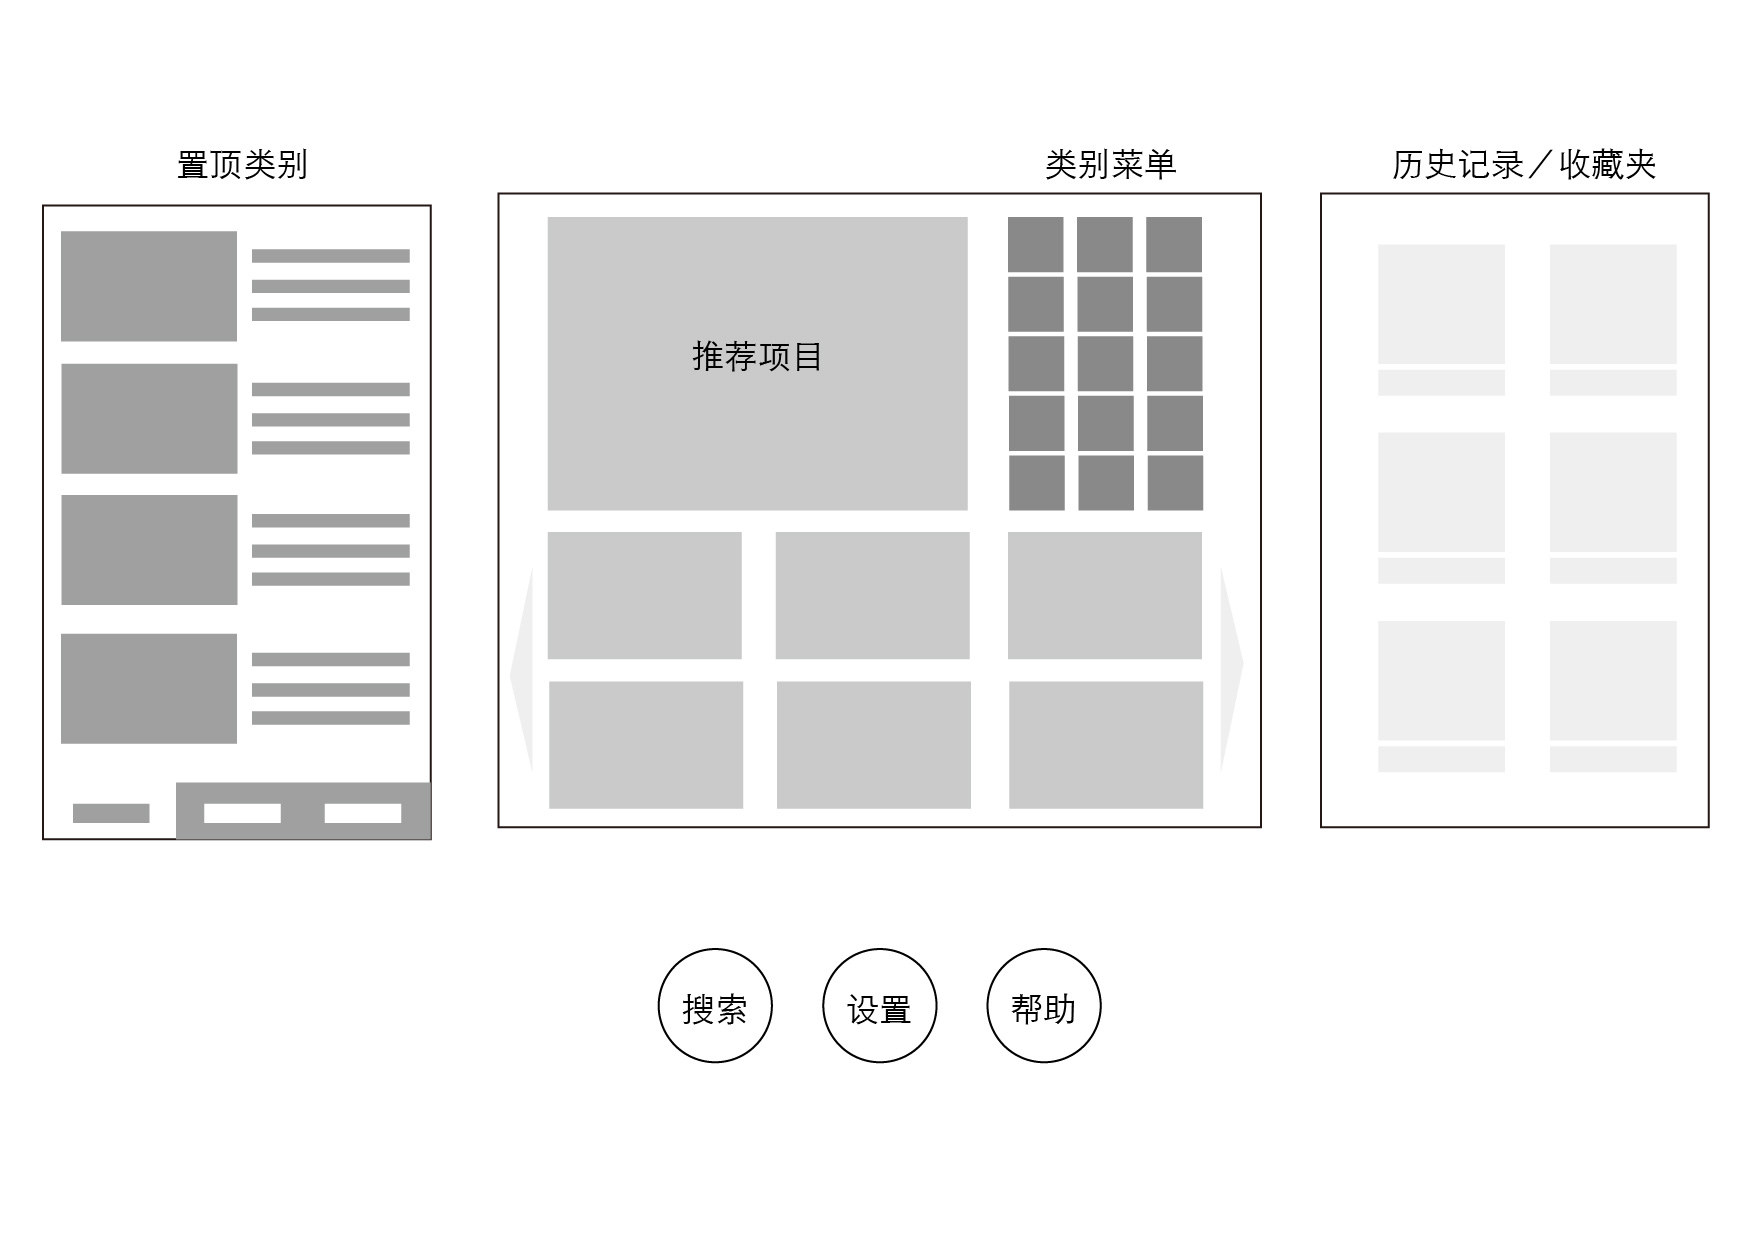
\includegraphics[width=.5\textwidth]{design/d-01}
}
\caption{主界面}
\label{fig:d-01}
\end{figure}

\subsubsection{类别界面}
类别界面则提供了更多分类以供选择,同时通过分页形式展示了全部的分类项目,考虑到用户操作次数的限制,通过筛选器查找分类里某个场景应用的功能意义较小,故在此只设计出以分类名查看场景应用的形式。分类的换页是不常用的功能,用户浏览的顺序大多为按类别查看第一页的项目,所以把分页设置于右侧,并且分页切换是上下排布,更利于用户通过仰头低头进行切换,降低了使用负担。类别界面如图\ref{fig:d-06}。

\begin{figure}[htp]
\centering
\fbox{
  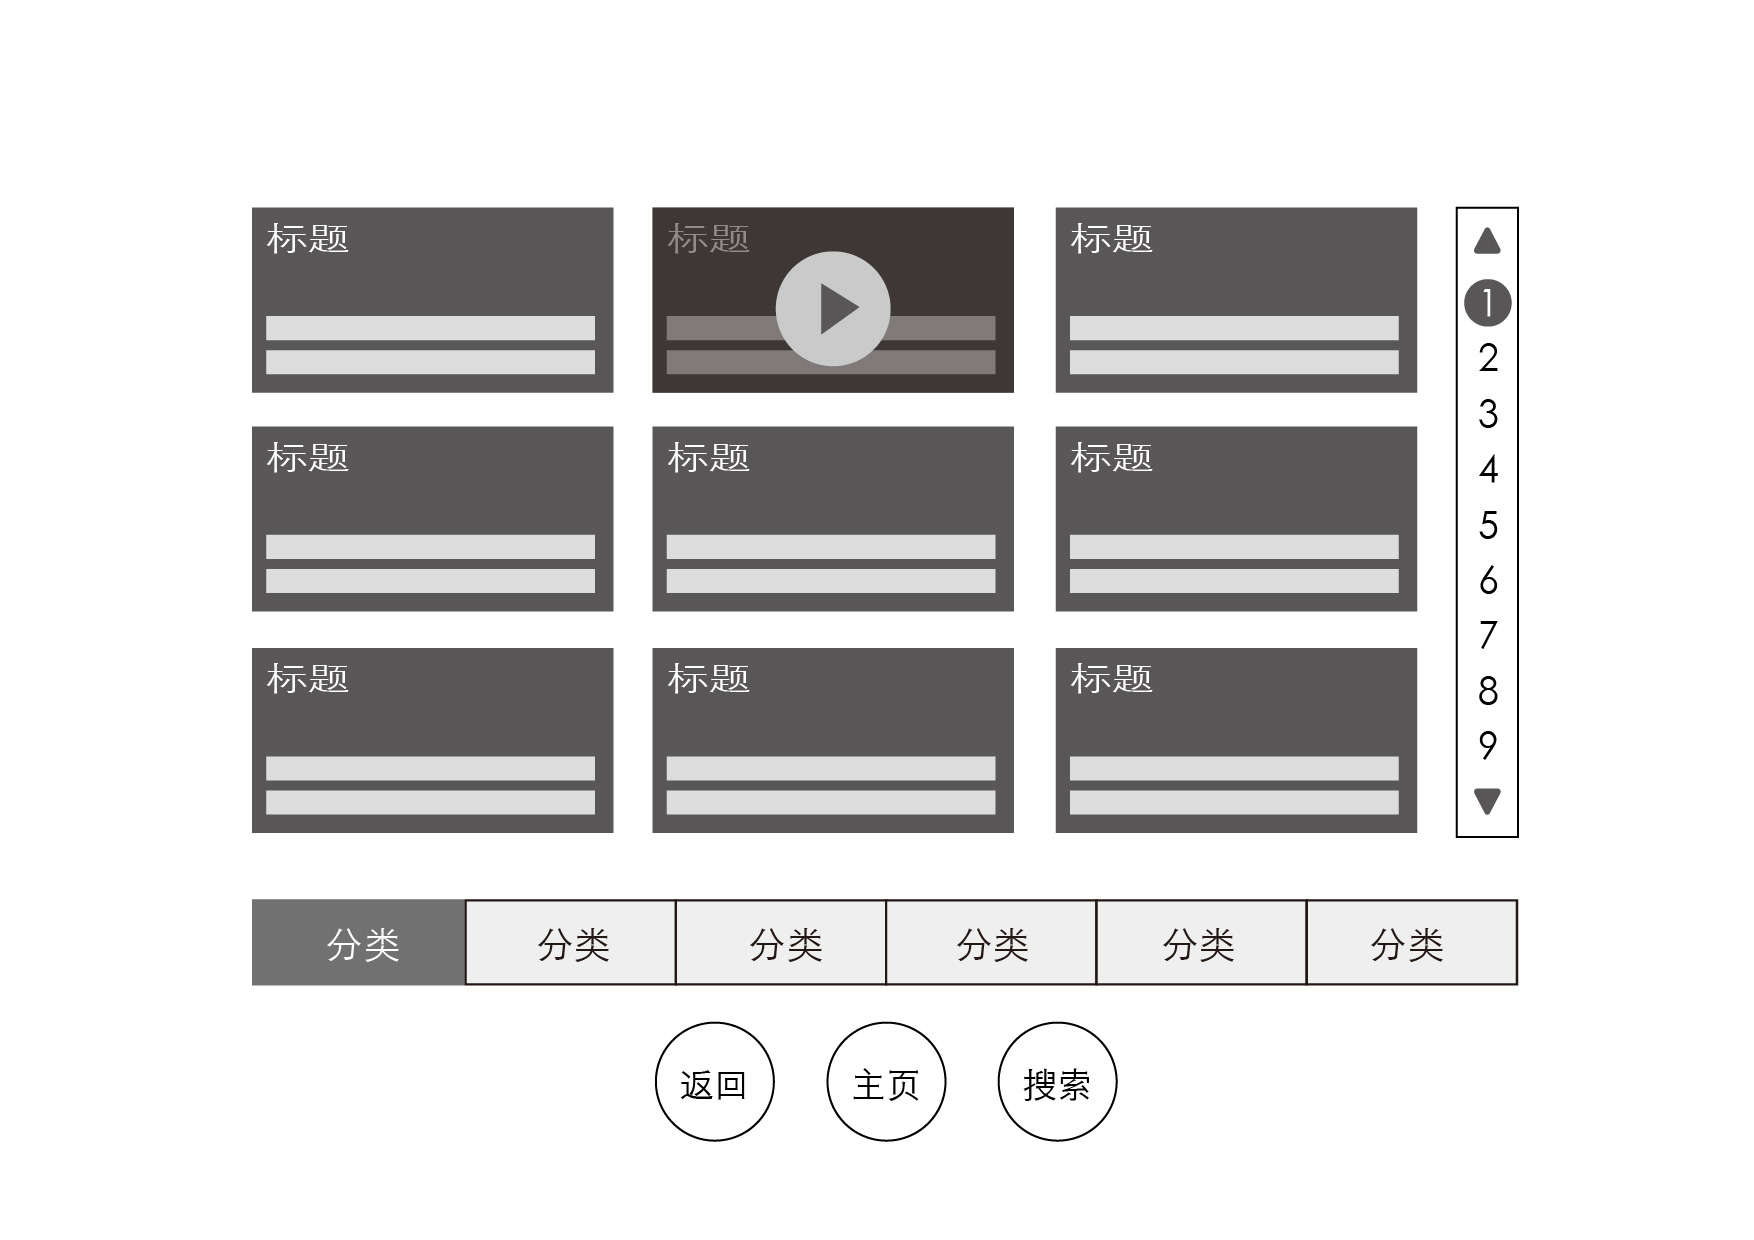
\includegraphics[width=.5\textwidth]{design/d-06}
}
\caption{类别界面}
\label{fig:d-06}
\end{figure}

考虑到存在用户偏向物理存在感强的菜单界面,故也有仿星系运动的界面如图\ref{fig:d-02}。这种界面趣味性更强,但因其与常见二维界面差别过大,开发难度和实现上难度较大,故本文只做示例,下文仍以平面导航界面为例说明。

\begin{figure}[htp]
\centering
\fbox{
  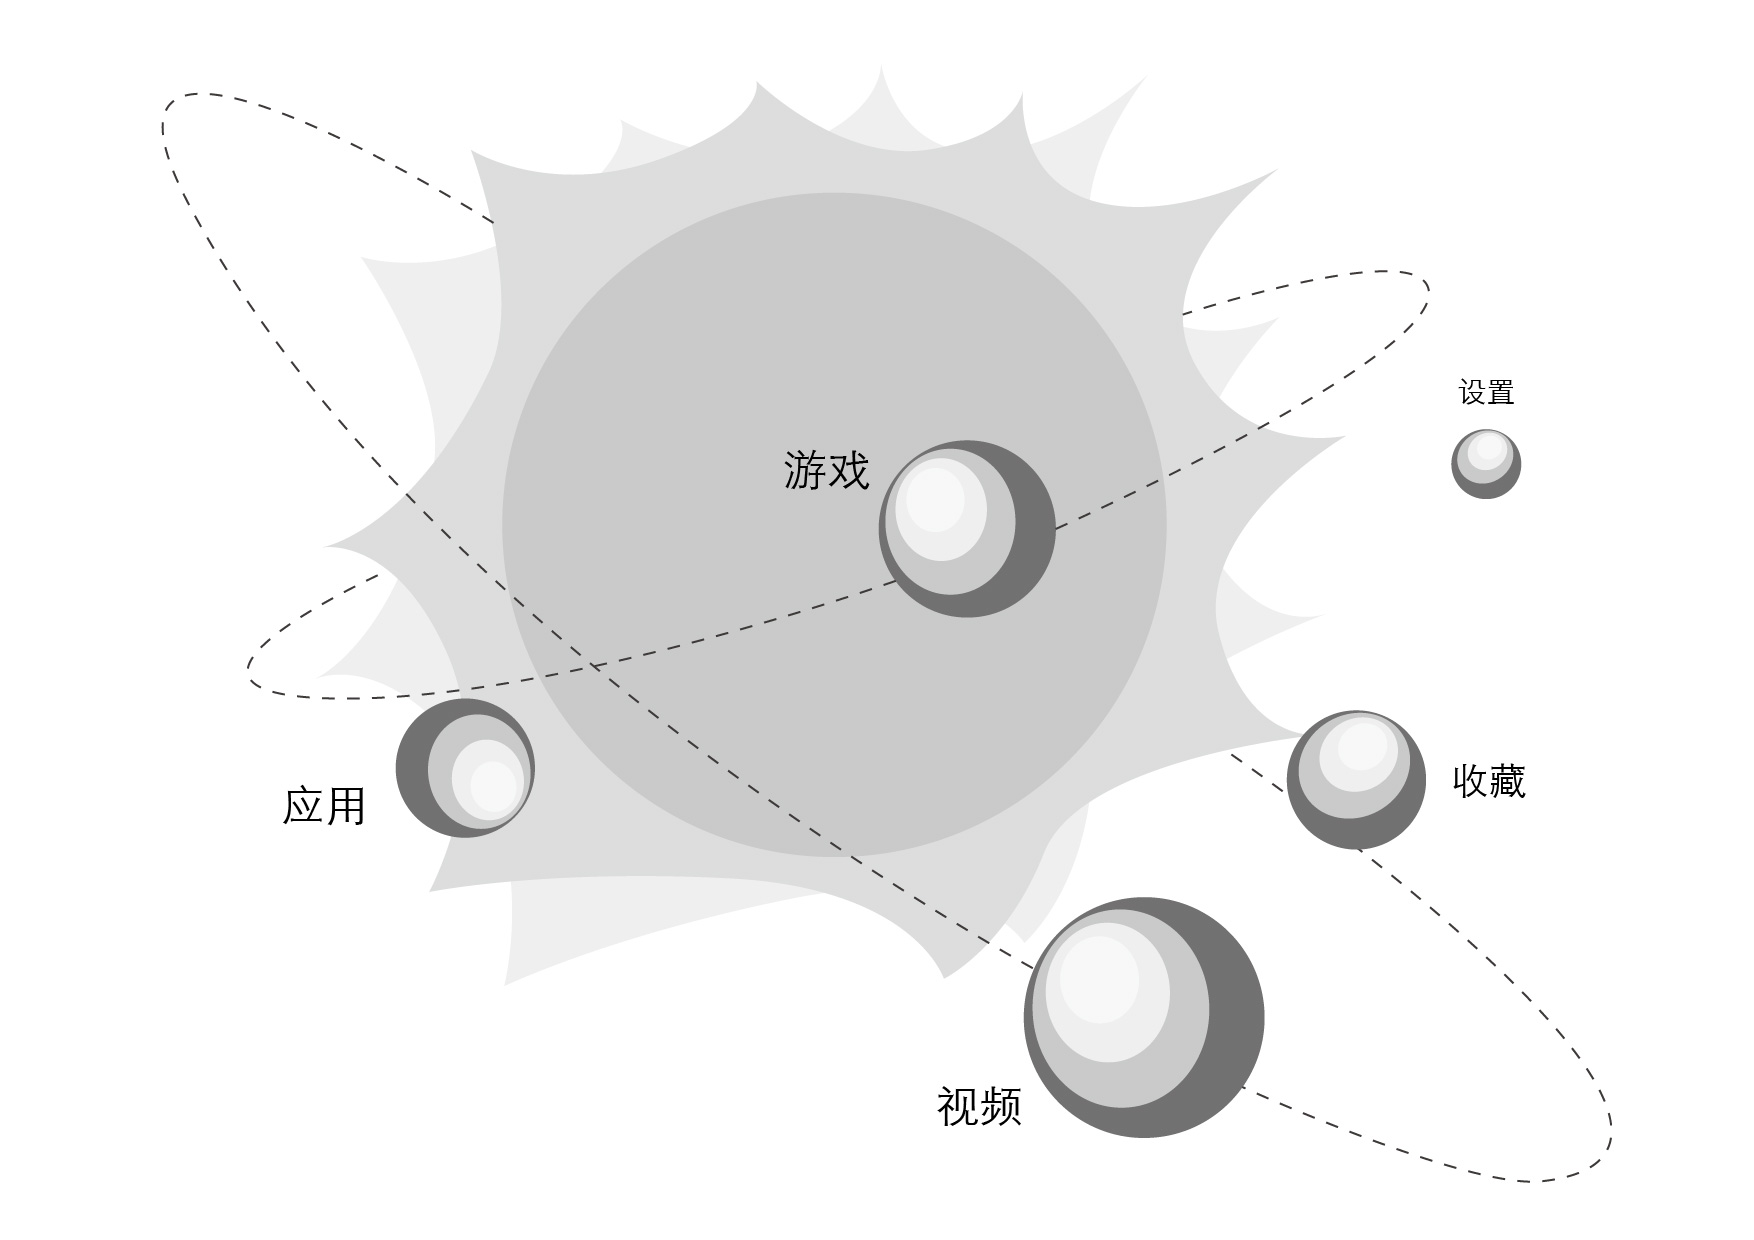
\includegraphics[width=.5\textwidth]{design/d-02}
}
\caption{星系状界面}
\label{fig:d-02}
\end{figure}

\subsubsection{详情界面}
详情界面是用户进入场景前的最后一个界面,这个界面的作用是在正式进入全景漫游应用前通过二维界面的形式,概括且有效地传递给用户场景相关的信息,帮助用户对全景场景建立模糊的信息架构。

该界面由三块相关的信息卡片构成。中心卡片为主卡片,介绍场景的基本信息,并包含“进入场景”、“收藏”和“分享”等三个功能按钮。主卡片的作用是引导用户进入场景或进行社交行为,故信息量较小。

左侧卡片为主观介绍信息,有图集、相关小知识和用户评价等三个模块,可以借助其他群体的图像文字资料让用户建立场景的第一印象。同时,用户也可在该卡片中分享自己对浏览该场景的体会。

右侧卡片为客观介绍信息,有地理信息、电话、好友标注等三个模块,帮助部分想要真正前往场景游玩的用户建立对真实场景的认识。其中,地理信息在该场景真实位置距用户较远时(不在同一国家)以三维地球形式展示,较近时(同一国家内)时以二维地图形式呈现。在该卡片中会显示同样对这个场景感心情的好友,方便用户结伴而行。

单个场景详情界面如图\ref{fig:d-07}。

\begin{figure}[htp]
\centering
\fbox{
  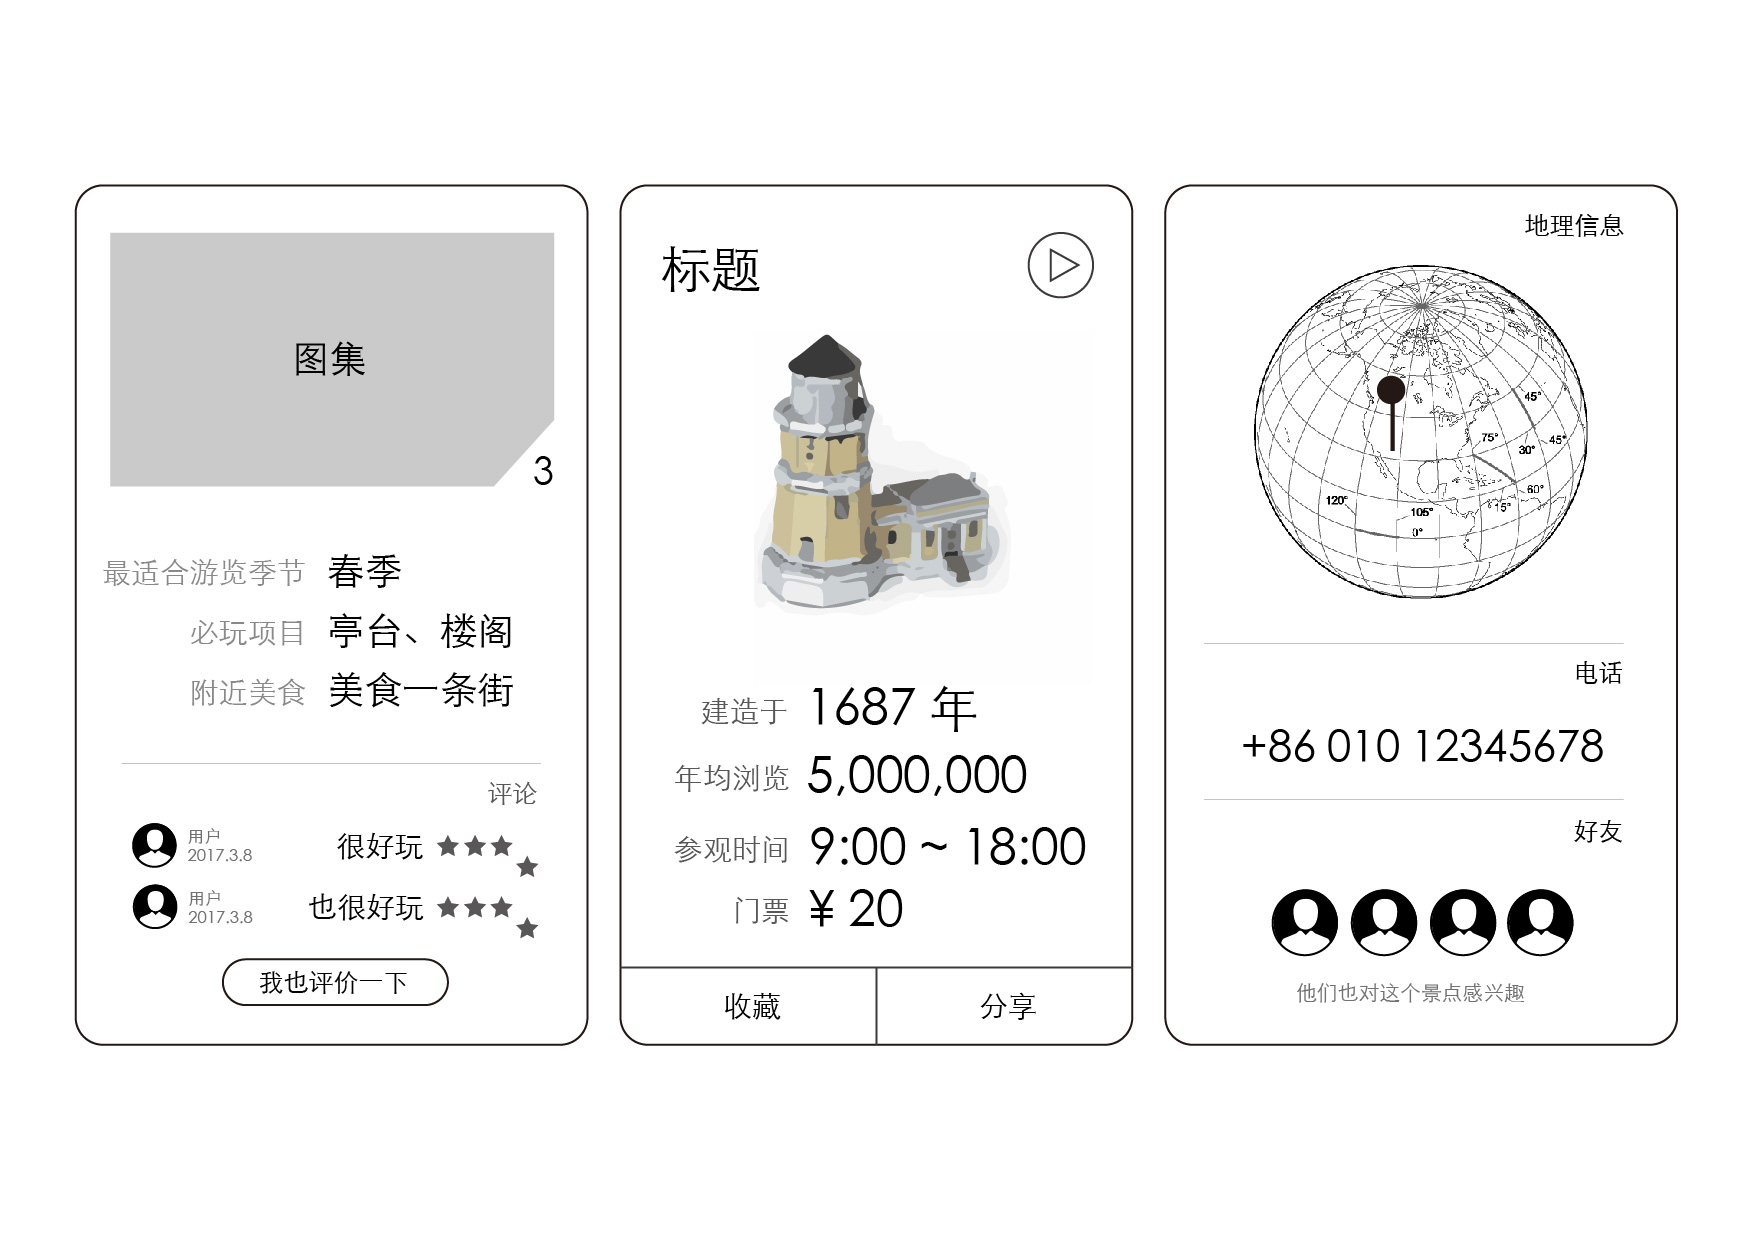
\includegraphics[width=.5\textwidth]{design/d-07}
}
\caption{单个场景详情界面}
\label{fig:d-07}
\end{figure}

\subsection{漫游界面设计}
\begin{itemize}
	\item 漫游界面带有紧急退出区域,只需视线停留 3 秒以上就可以紧急退出场景,避免眩晕加重。
	\item 可通过地面上的指示图标切换场景。
	\item 可通过场景中的热点区域查看详细信息。
\end{itemize}

设置紧急退出的区域的目的是防止用户因长时间处于紧张及刺激状态造成晕眩,此时用户精神难以集中,若继续采取普通的凝视触发按钮触发退出的操作形式,用户操作失败率会变高很多,应转换为更大面积且更容易触发的形式。此时,用户只需仰头数秒,就可退出全景漫游应用乃至直接关闭设备。
如图\ref{fig:scenery}。

\begin{figure}[htp]
\centering
\fbox{
  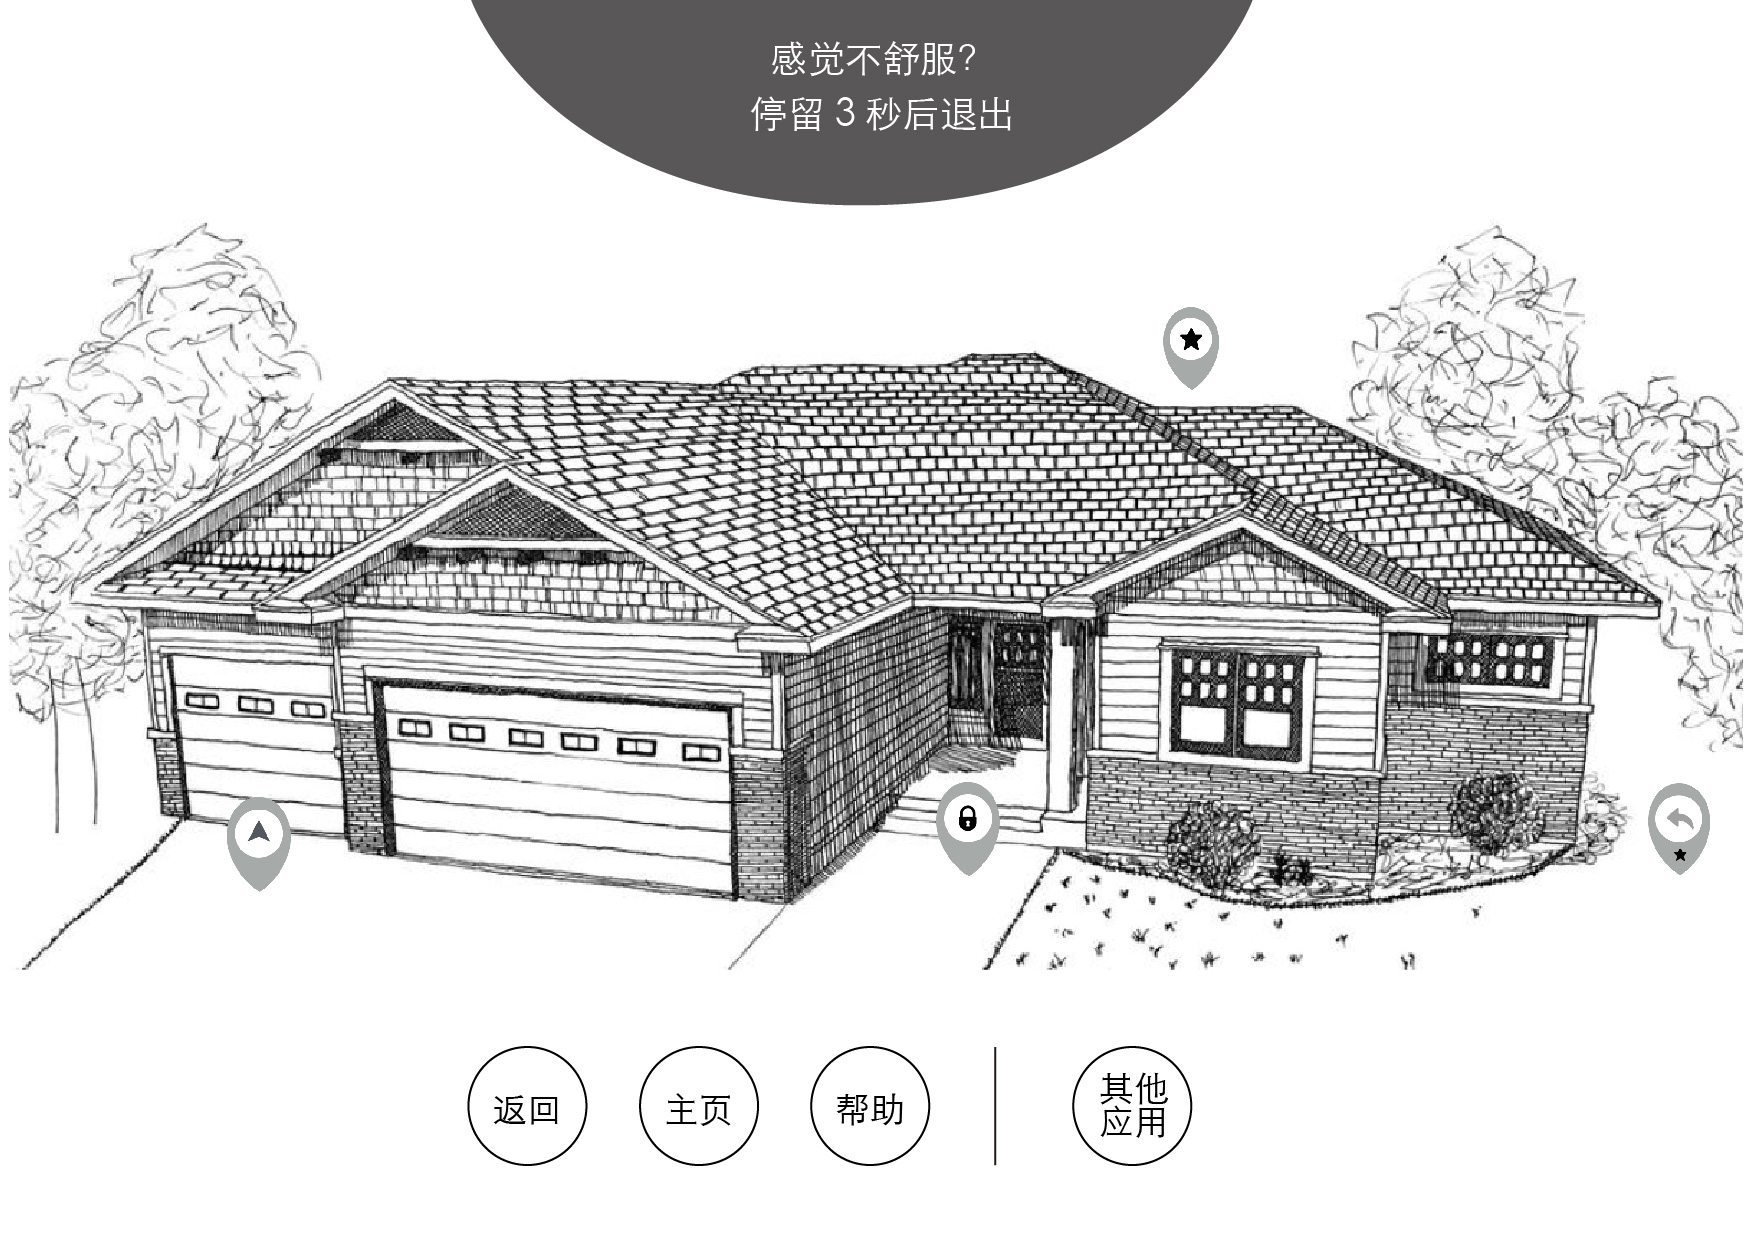
\includegraphics[width=.5\textwidth]{design/d-08}
}
\caption{漫游界面设计}
\label{fig:scenery}
\end{figure}

在漫游中使用四向盘进行镜头的位移\endnote{李海洋,范文义,李明泽. 二维地图与三维虚拟场景交互技术的研究与应用[J]. 东北林业大学学报,2008,(11):92-94.},如图\ref{fig:d-10}。具体交互形式见下文的漫游操作方式设计。

\begin{figure}[htp]
\centering
\fbox{
  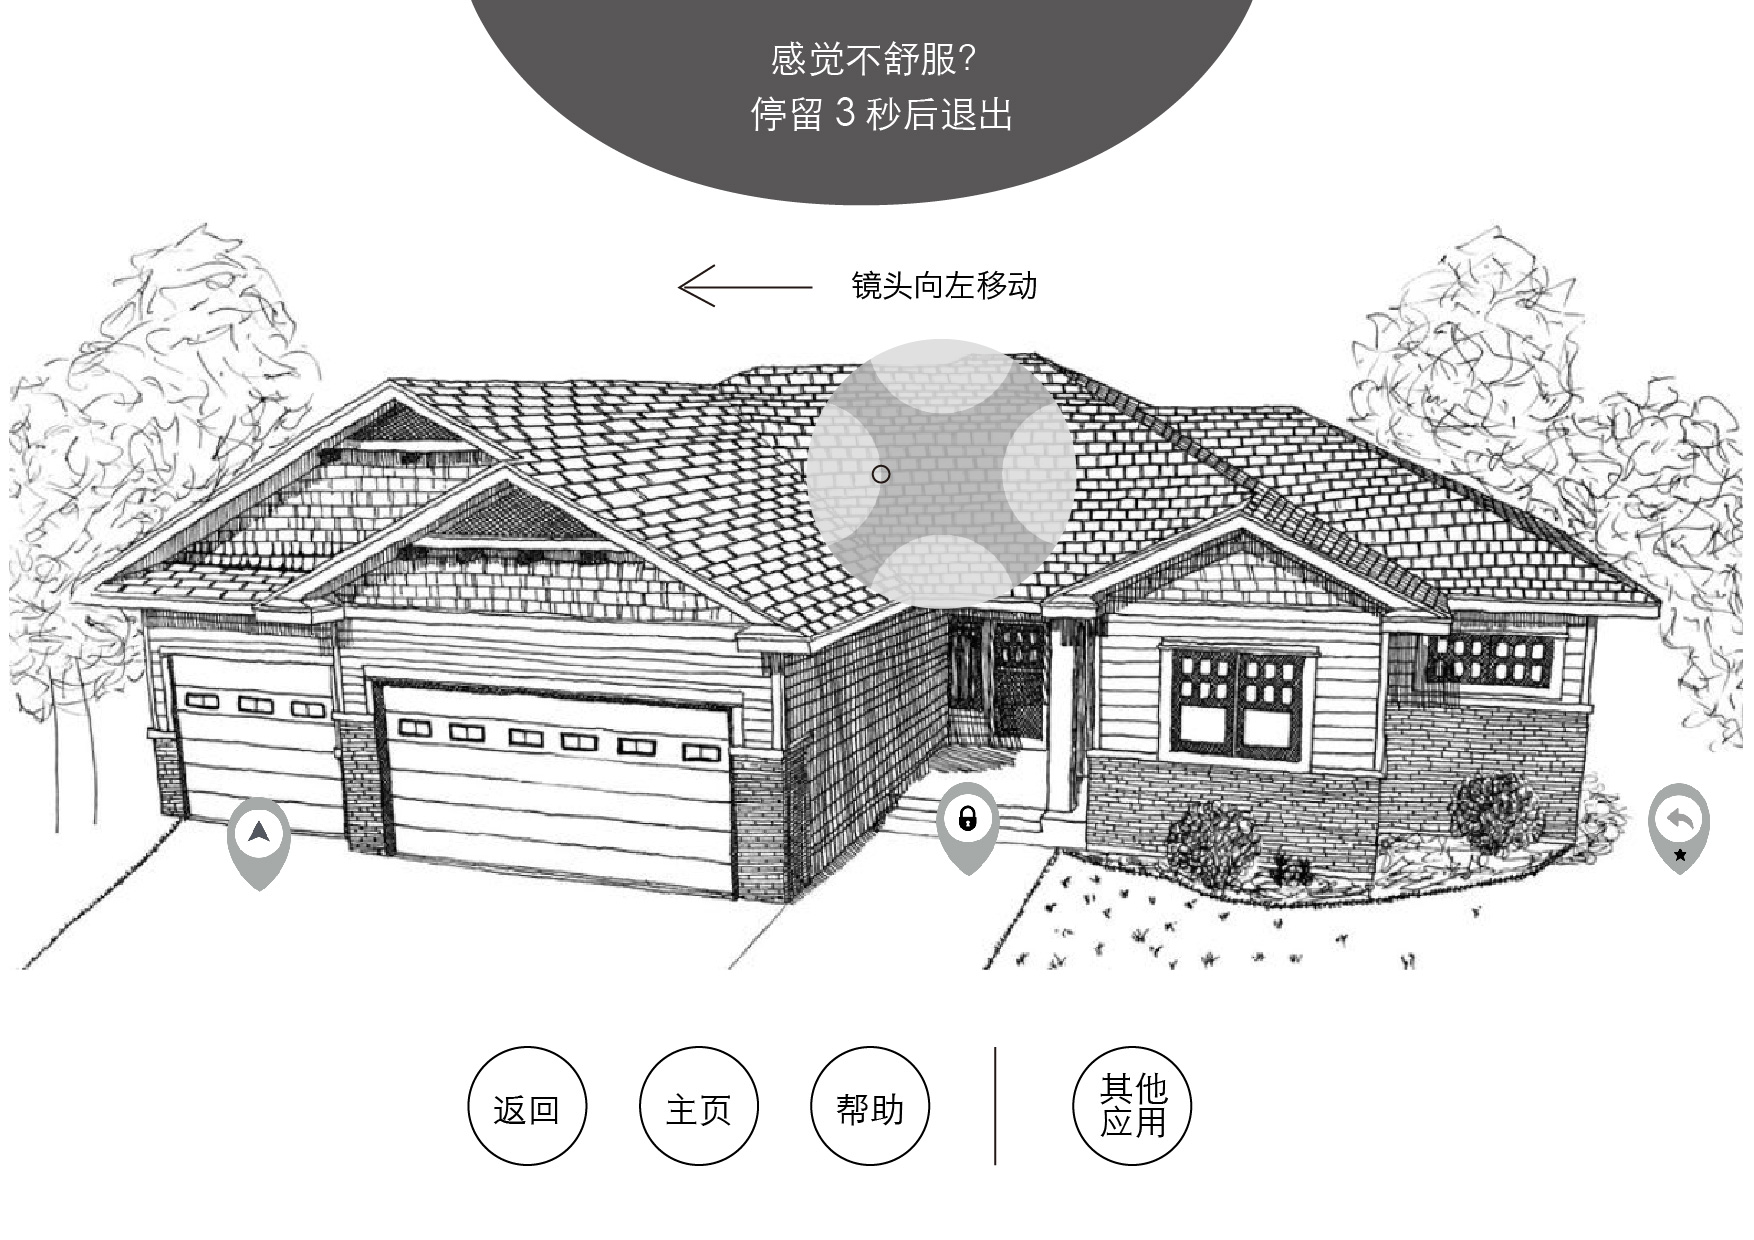
\includegraphics[width=.5\textwidth]{design/d-10}
}
\caption{漫游中进行镜头位移}
\label{fig:d-10}
\end{figure}

当漫游场景中字场景数量多并且相互逻辑不够清晰时,可采用将场景缩略图置于视野上方悬浮的形式以作参考,如图\ref{fig:d-11}。

\begin{figure}[htp]
\centering
\fbox{
  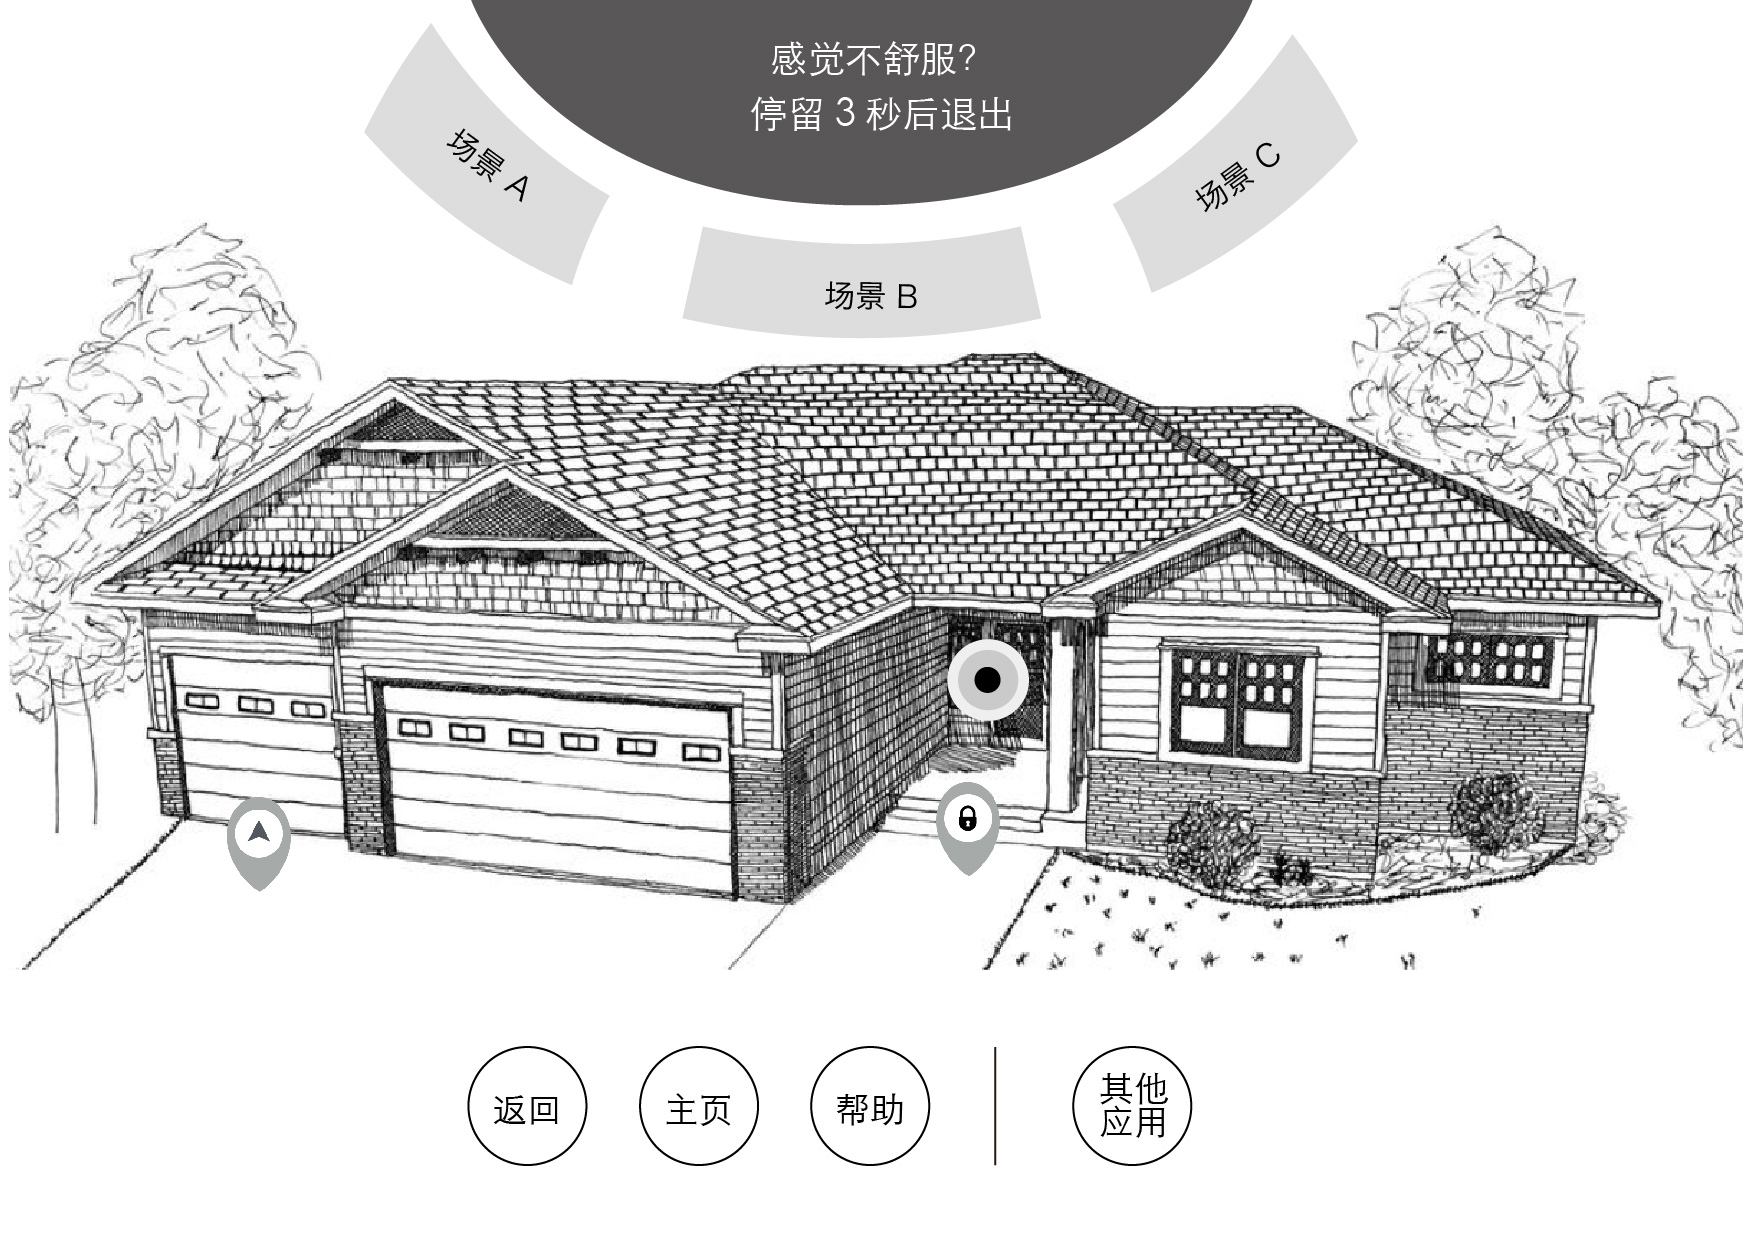
\includegraphics[width=.5\textwidth]{design/d-11}
}
\caption{漫游中场景缩略图}
\label{fig:d-11}
\end{figure}

\subsection{功能界面设计}

功能界面是为了满足特定功能需要而区别于一般列表详情等的特殊界面,其设计在符合整体设计规划的同时也具有特异性,表现为侧重于满足特殊功能的特殊交互形式或控件。以下介绍语音搜索、设置及支付等三种特殊界面等原型设计。

\subsubsection{语音搜索}
语音搜索界面,左侧上方为语音控件,凝视触发后可以采集声音经识别后转换为文字,在其下文本框内可以看到识别后的文字。右侧为根据所识别等文字所推荐的选项,因语音输入识别仍存在输入效率低的问题,故推荐选项可以一定程度上提升用户一次性输入符合预期的搜索文字的成功率。语音搜索界面如图\ref{fig:d-04}。

\begin{figure}[htp]
\centering
\fbox{
  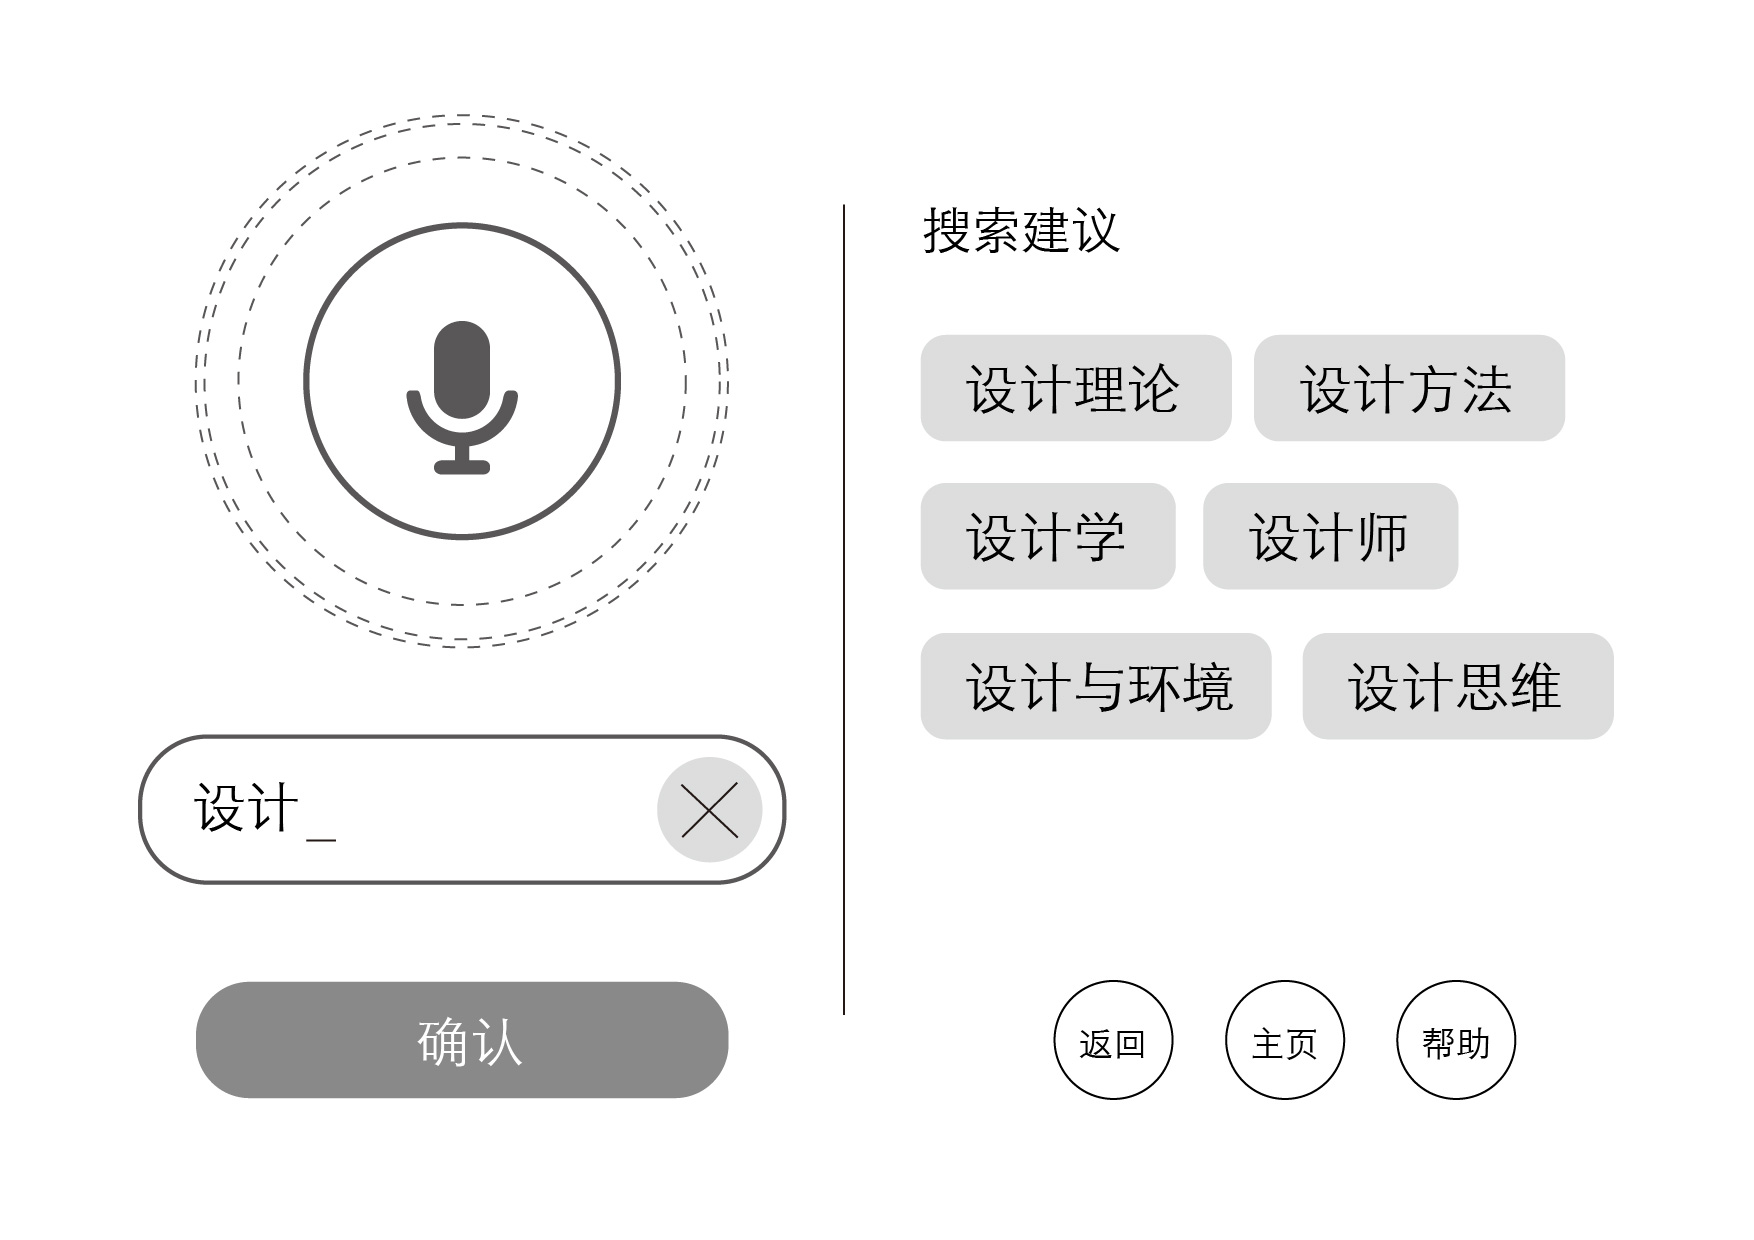
\includegraphics[width=.5\textwidth]{design/d-04}
}
\caption{语音搜索界面}
\label{fig:d-04}
\end{figure}

\subsubsection{设置界面}
设置界面提供用户对系统整体布局的调整选项。布尔选项框的操作方式于按钮类似,都为凝视触发。范围选择控件的触发方式为视线凝视后定位到指定位置,在视线经过时也会提示当前视线位置的刻度值。设置界面如图\ref{fig:d-05}。

\begin{figure}[htp]
\centering
\fbox{
  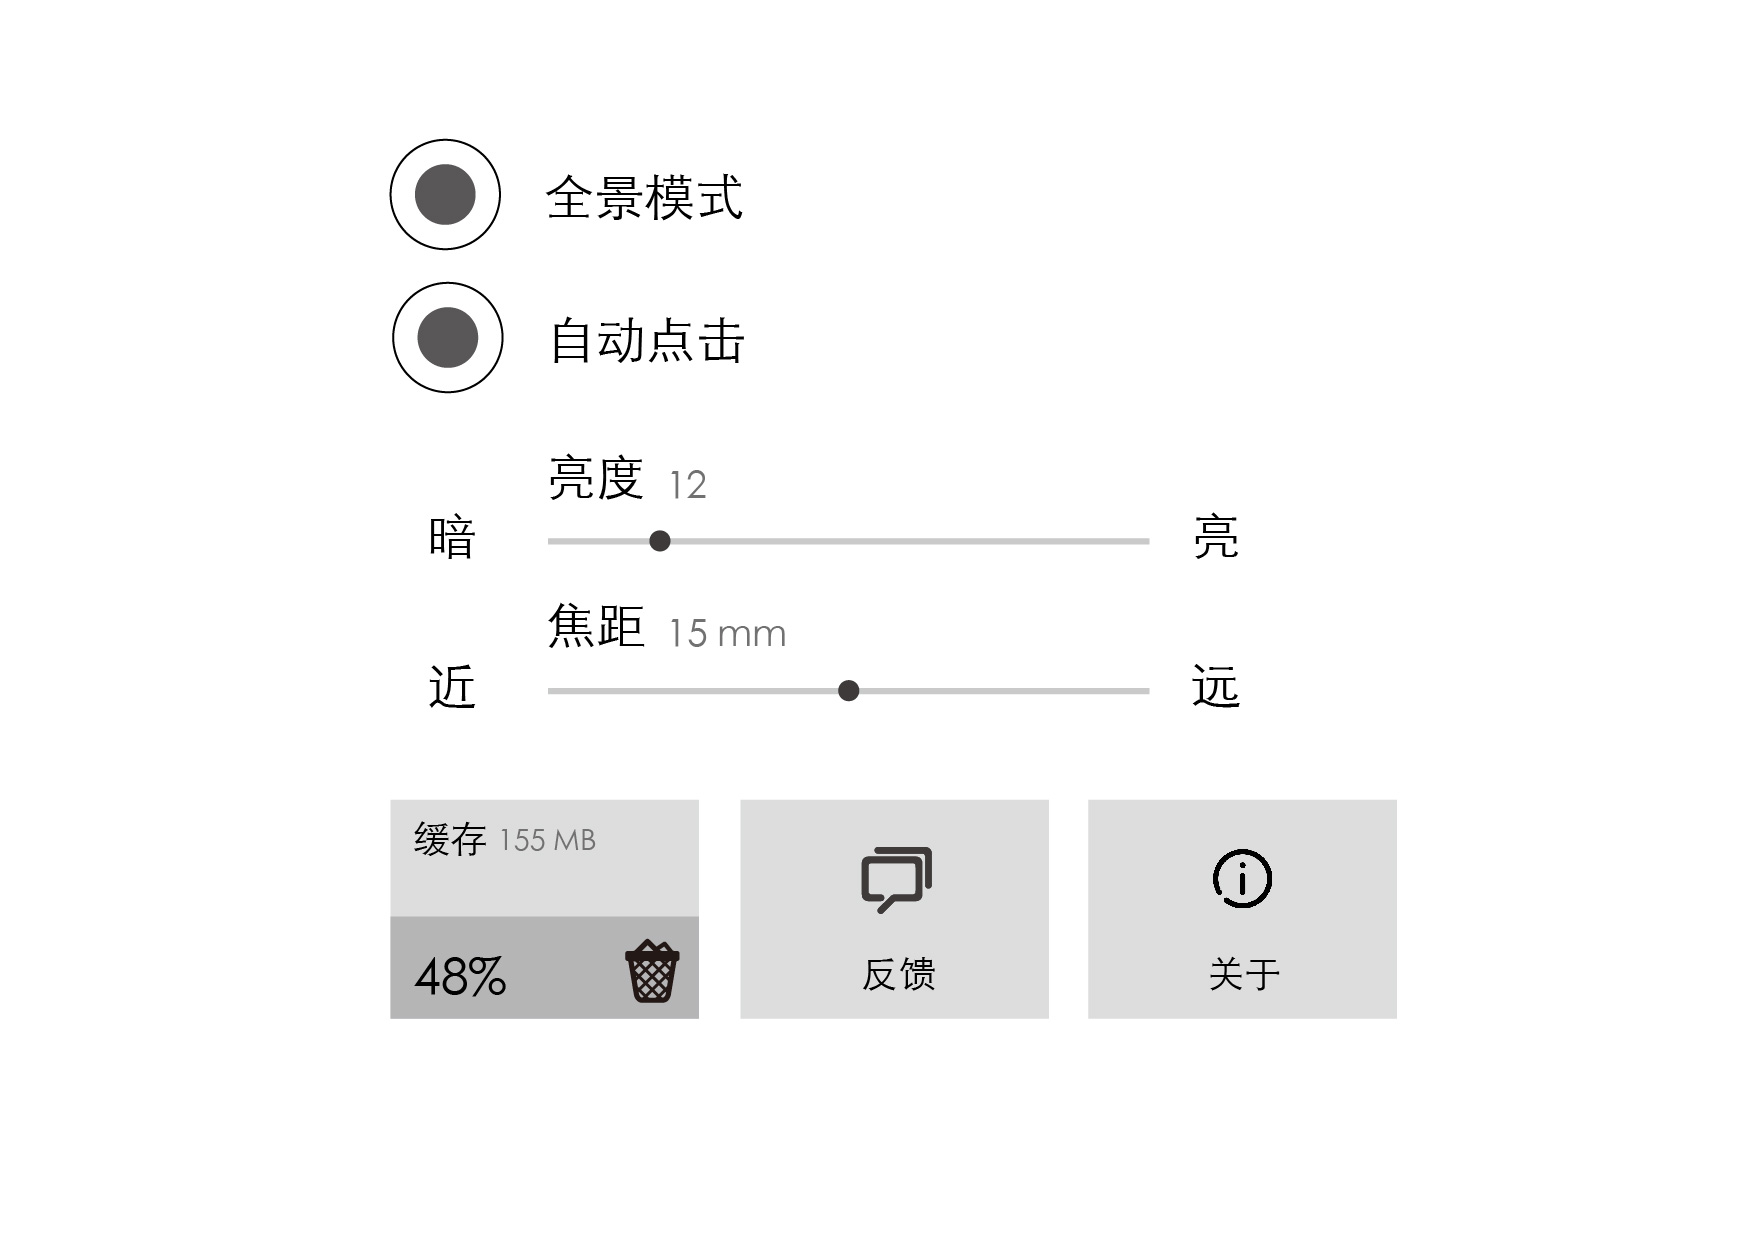
\includegraphics[width=.5\textwidth]{design/d-05}
}
\caption{设置界面}
\label{fig:d-05}
\end{figure}

\subsubsection{支付界面}
支付界面显示了购买项目、金额等基本信息,同时提供了支付方式和支付密码两项需要用户输入的控件。用户需要确认支付的内容,以及根据需要选择支付方式,并通过密码验证,最后在右侧选择“确认支付”或是“取消支付”选项。

考虑到用户在连续输入两项后易因注意分散而产生误操作的可能,将确认取消按钮置于右侧后需要用户头部偏转才可以完成全部支付流程。确认步骤需要用户将视线先向右偏转,再上下浏览选项进行思考,客观上增加了操作的局部复杂度,有助于用户调整注意力,减少错误操作的概率\endnote{钱程. 微交互在B2C网站界面设计中的应用与研究[D].湖北工业大学,2016.}。

支付界面如图\ref{fig:d-12}。

\begin{figure}[htp]
\centering
\fbox{
  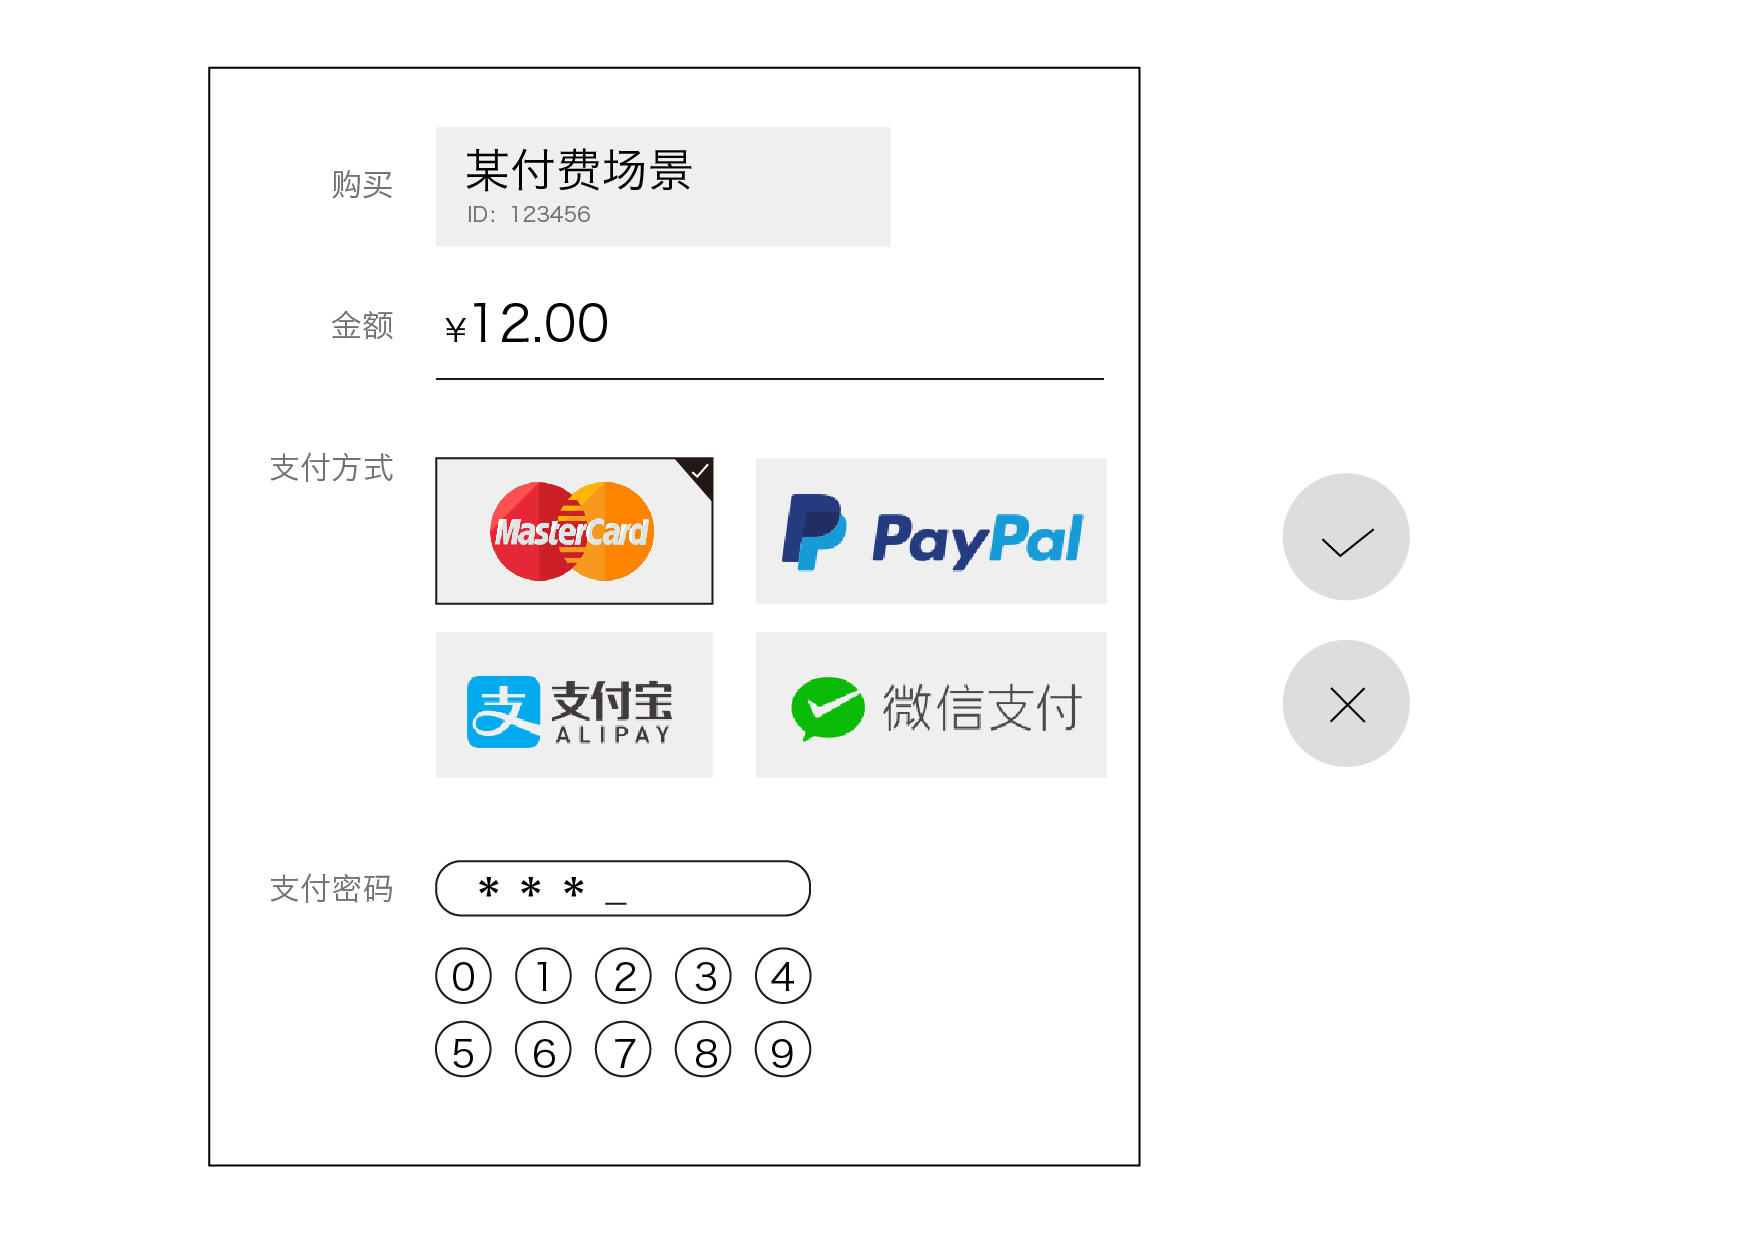
\includegraphics[width=.5\textwidth]{design/d-12}
}
\caption{支付界面}
\label{fig:d-12}
\end{figure}

\subsection{操作方式设计}

凝视触发是普通按钮和位移控件的基本触发形式,在图\ref{fig:d-09}中加以说明。

前翻和后翻功能是类似书本翻页的功能,可以被用户较为轻松地理解为场景的切换功能,但场景的切换一般为通过触发场景内特定指向箭头,不宜于用户直观寻找,故设置前翻或后翻控件,当视线短时二次进入时可触发切换场景(类似于翻页)的操作,其设计借鉴于移动端场景漫游中上下拖动切换场景的操作\endnote{赵晓倩,王晨升,陈亮,王冬冬. 移动端三维界面两种交互方式的比较研究[J]. 产业与科技论坛,2012,(15):80-81.}。因全景漫游中上下空间被导航栏使用,左右摆头可能为更适合全景漫游切换场景的方式,同时考虑操作中的容错率,快速摆头至指定区域两次可视为一次完整的头部动作,从而触发切换场景的操作。
操作方式示意如图\ref{fig:d-09}。

\begin{figure}[htp]
\centering
\fbox{
  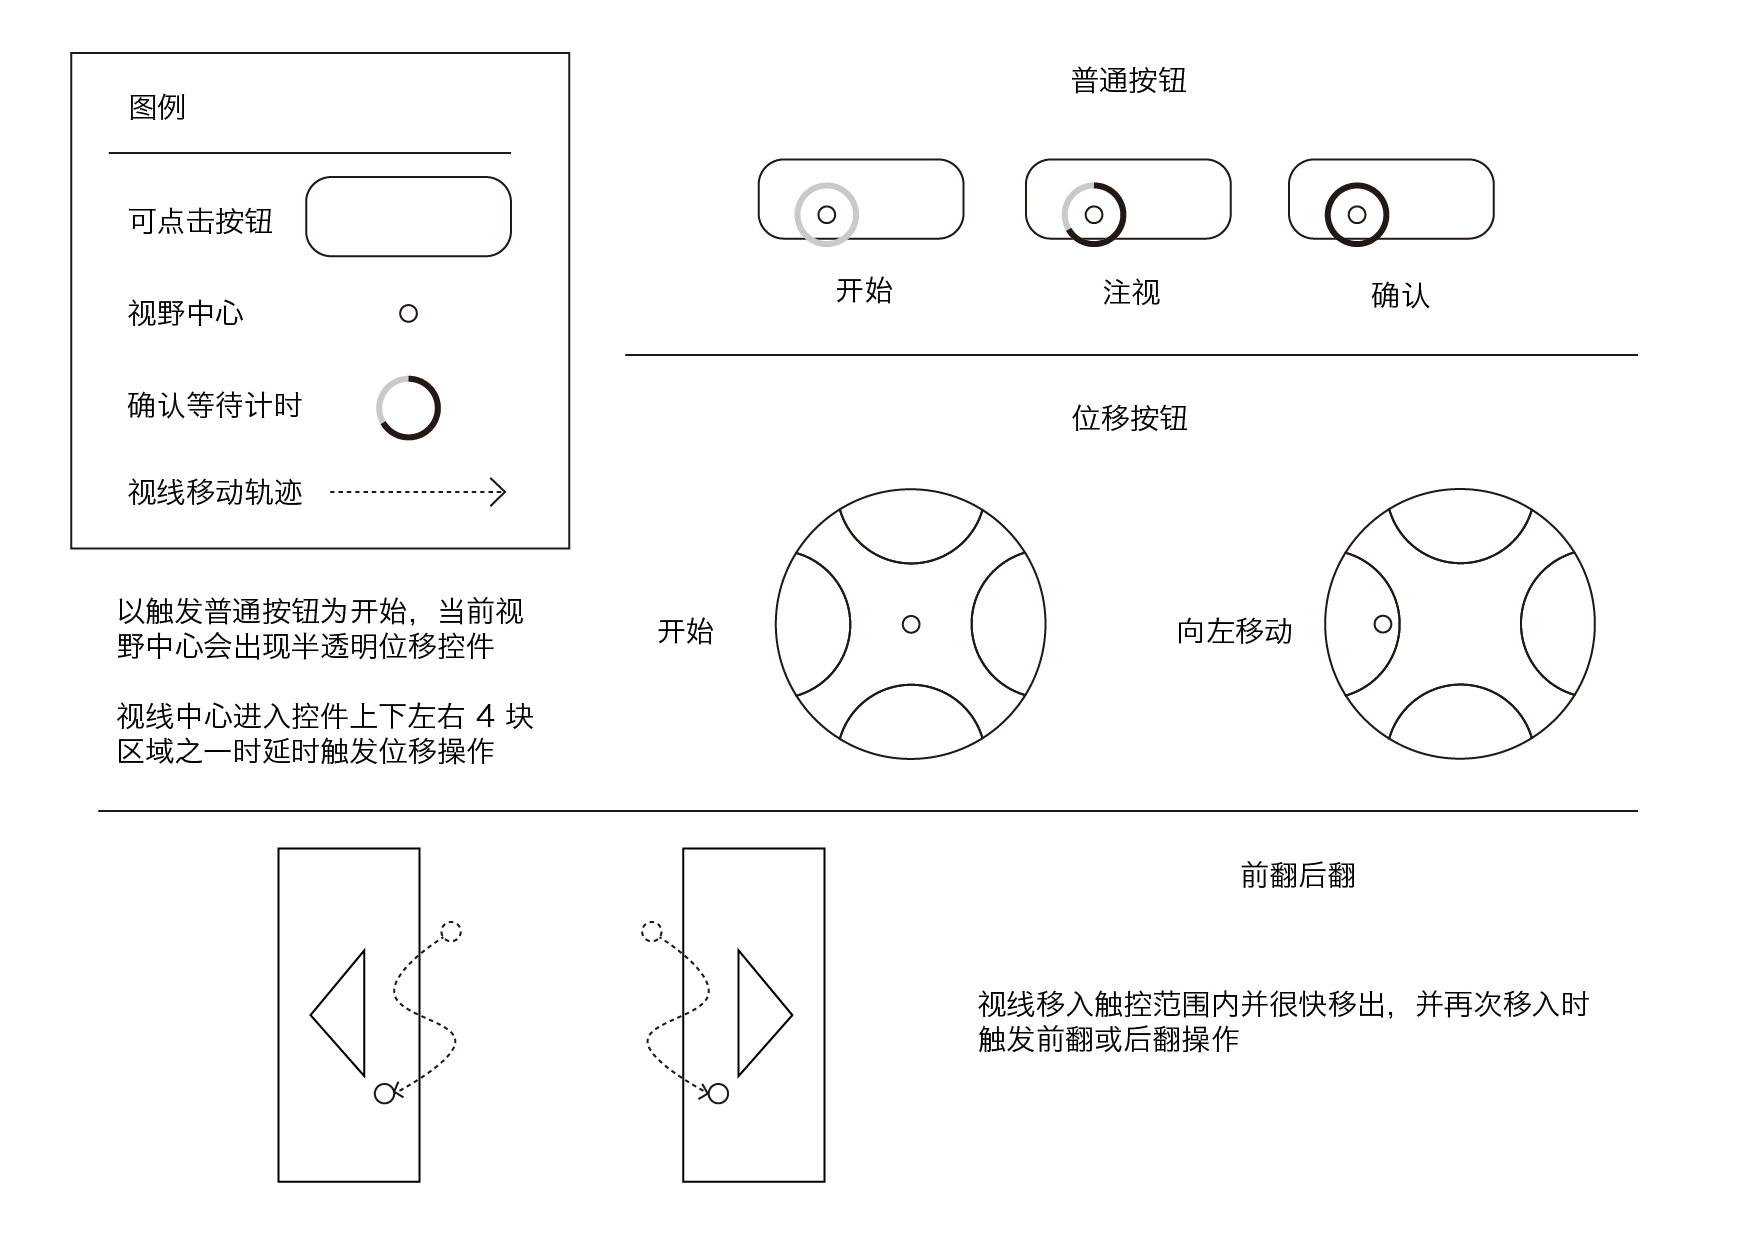
\includegraphics[width=.9\textwidth]{design/d-09}
}
\caption{操作方式示意}
\label{fig:d-09}
\end{figure}